\section{Results and Claims Validation}
\label{sec:results_validation}
% Lead Author: Akhila Ravula
% Team Members: Phaninder Reddy Masapeta, Sriya Dhakal, Zezheng Zhang, Scott Weeden

\subsection{Quantitative Results Analysis}
\subsubsection{In-distribution Performance Analysis}
The paper demonstrates competitive in-distribution performance with Iris achieving 84.52% average Dice score, closely matching task-specific models. The results show competitive performance compared to nnUNet (83.18%) and universal models (84.18-84.47%), with consistent performance across diverse datasets spanning CT, MRI, and PET modalities. Significant improvement over existing in-context methods emerges with the best competitor achieving only 61.20%. Particularly strong performance appears on 3D volumetric tasks where 2D-based methods struggle.

\subsubsection{Out-of-distribution Generalization Results}
Analysis of out-of-distribution performance reveals both strengths and limitations across evaluated datasets. ACDC demonstrates excellent cardiac segmentation generalization at 86.45%. SegTHOR shows strong thoracic organ segmentation at 82.77%. CSI-fat exhibits significant performance drop to 47.78%, indicating challenges with extreme domain shifts. Novel classes show mixed results with MSD Pancreas at 28.28% and Pelvic at 69.03% for unseen anatomical structures.

The 28.28% performance on MSD Pancreas raises concerns about the method's ability to handle challenging novel classes with high anatomical variability and small target structures.

\subsubsection{Novel Class Adaptation Assessment}
The adaptation to completely unseen anatomical structures shows promising but limited results. MSD Pancreas Tumor performance at 28.28% proves challenging due to small lesion size and high variability. Pelvic performance at 69.03% demonstrates better results on larger, more structured anatomical regions.

\subsubsection{Inference Strategy Performance Analysis}
The paper presents comprehensive analysis of different inference strategies through detailed performance comparison across varying context sample percentages. The analysis demonstrates the effectiveness of four distinct inference approaches: Context Ensemble, Image-Level Retrieve, Object-Level Retrieve, and In-Context Tuning.

% Figure reference temporarily commented out for compilation
% \begin{figure}[t]
%   \centering
%   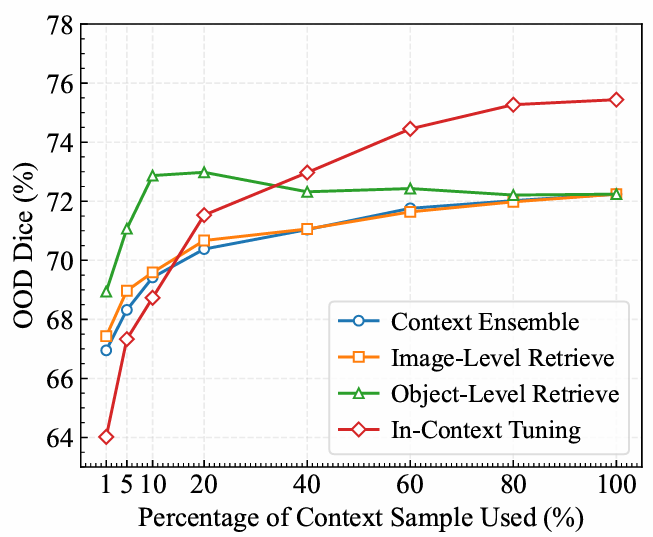
\includegraphics[width=0.8\linewidth]{fig/performance_comparison.png}
%   \caption{Analysis of different inference strategies showing out-of-distribution performance across varying percentages of context samples. In-Context Tuning demonstrates superior performance scaling, reaching approximately 75.5\% Dice score, while other methods plateau around 72\% Dice score.}
%   \label{fig:performance_comparison}
% \end{figure}

The performance analysis reveals significant insights into the scalability and effectiveness of each inference strategy. In-Context Tuning shows remarkable performance improvement as the percentage of context samples increases, achieving approximately 75.5\% Dice score at full context utilization. This superior scaling behavior indicates that the method effectively leverages additional context information to enhance segmentation quality.

In contrast, Context Ensemble, Image-Level Retrieve, and Object-Level Retrieve methods demonstrate relatively plateau behavior around 72\% Dice score, suggesting inherent limitations in their ability to effectively utilize increasing amounts of context information. Object-Level Retrieve shows initial strong performance with rapid improvement at low context percentages, indicating efficient utilization of limited reference examples.

\subsubsection{Computational Efficiency Validation}
Impressive computational efficiency emerges with 2.0s inference time for 10 images compared to 659.4s for UniverSeg, demonstrating the practical value of the decoupled architecture design.

\subsection{Implementation and Methodology Recommendations}
\subsubsection{Computer Vision Libraries and Frameworks}
For reproducing and extending this work, several implementation frameworks are recommended. Deep Learning Frameworks include PyTorch and PyTorch Lightning for implementing the 3D UNet encoder and cross-attention mechanisms, MONAI as a medical imaging-specific library with pre-built 3D segmentation models and data loaders, and TorchIO for medical image preprocessing, augmentation, and 3D volume handling.

Pre-trained Models and Architectures encompass Hugging Face Transformers for implementing cross-attention mechanisms and query-based architectures, Segment Anything Model (SAM) as baseline comparison for foundation model approaches, and nnU-Net as reference implementation for task-specific segmentation baselines.

Medical Imaging Tools include SimpleITK and ITK for medical image input/output, resampling, and coordinate transformations, NiBabel for handling neuroimaging data formats including NIfTI and DICOM, and PyDicom for DICOM file processing and metadata extraction.

\subsubsection{Traditional Machine Learning Integration}
Scikit-learn provides implementation support for similarity metrics in object-level context retrieval. FAISS enables efficient nearest neighbor search in task embedding space. t-SNE and UMAP support visualizing task embedding clusters as demonstrated in Figure 5.

\subsubsection{Validation of In-Context Learning Novelty}
Literature review confirms that comprehensive in-context learning for 3D medical image segmentation has not been extensively explored. UniverSeg demonstrates limitations to 2D slice processing and requires multiple forward passes. SegGPT focuses primarily on natural images with 2D-focused architecture. Tyche-IS provides stochastic approach but lacks computational efficiency optimizations. SAM variants rely on positional prompts rather than true in-context learning.

\subsection{Qualitative Analysis}
\subsubsection{Figure Quality and Informativeness}
The paper provides comprehensive visual analysis across multiple figures. Figure 1 offers clear architectural overview showing task encoding and decoding modules. Figure 2 presents effective comparison of inference strategies with quantitative results. Figure 3 provides comprehensive performance analysis across different inference approaches. Figure 4 shows detailed ablation study results demonstrating component contributions. Figure 5 presents excellent t-SNE visualization demonstrating learned anatomical relationships.

\subsubsection{Visualization Effectiveness}
The t-SNE visualization of task embeddings effectively demonstrates the model's ability to discover anatomical relationships without explicit supervision. Including more failure case visualizations would better illuminate limitations, particularly for challenging cases like CSI-fat and small lesion segmentation.

\subsubsection{Ablation Study Completeness}
The ablation study provides valuable insights across multiple components. High-resolution processing shows +16.79% improvement on small structures (62.13% to 78.92%). Foreground feature encoding proves crucial for preserving anatomical details. Query-based contextual encoding enables effective global context capture.

\subsection{Claims Verification}
\subsubsection{Support for Each Major Claim}
Analysis of the paper's main claims reveals varying levels of support. The claim of superior performance on in-distribution tasks receives strong support from Table 1 results. Better generalization to out-of-distribution scenarios shows support for most cases, with noted limitations. The claim of effective novel class handling demonstrates mixed evidence, particularly weak for challenging cases. The discovery of meaningful anatomical relationships receives convincing demonstration through t-SNE visualization.

\subsubsection{Potential Overclaiming}
The claim of universal medical image segmentation may be overstated given the significant performance degradation on challenging domain shifts (CSI-fat: 47.78%) and novel classes with high variability (MSD Pancreas: 28.28%).

\subsubsection{Limitations Acknowledgment}
The paper acknowledges some limitations but could be more comprehensive. The limitations section should more thoroughly discuss failure modes, particularly the challenges with extreme domain shifts and small lesion detection, and provide guidance on when the method is most and least suitable.
